\documentclass[a4paper, 12pt, fleqn]{article}
\usepackage[utf8]{inputenc}
\usepackage{graphicx}
\usepackage[T1]{fontenc}
\usepackage{amssymb}
\graphicspath{ {images/} }
\usepackage[a4paper,left=.8in,right=.8in,top=1in,bottom=1in]{geometry}
\setlength\oddsidemargin{\dimexpr(\paperwidth-\textwidth)/2 - 1in\relax}
\setlength\evensidemargin{\oddsidemargin}
%\setlength\oddsidemargin{-.875in}
%\setlength\evensidemargin{-.875in}
\usepackage{tikz}
\usetikzlibrary{positioning,shapes,fit,arrows}
\definecolor{myblue}{RGB}{56,94,141}
\usepackage{fancyhdr}
\usepackage{booktabs}
\usepackage{mathtools}
\usepackage{amsmath}
\usepackage{etoolbox}
\usepackage[hidelinks]{hyperref}
%\apptocmd{\thebibliography}{\csname phantomsection \endcsname \addtocontentsline{toc}{chapter}{\bibname}}{}{}
\usepackage{caption}
\usepackage{float}
\floatstyle{boxed} 
\restylefloat{figure}
\pagestyle{fancy}
\fancyhf{}
\fancyhead[LE,RO]{}
\fancyfoot[CE,CO]{}
\fancyfoot[LE,RO]{\thepage}

\begin{document}
 
\begin{titlepage}
    \begin{center}
        \vspace*{1cm}
        \par
        \large
                \textbf{Pune Institute of Computer Technology}	
                \linebreak
		\textbf{Dhankawadi, Pune}
        \vspace{0.5cm}
        \linebreak
        \vspace{0.5cm}
        \large
        \\Greg Viot's Fuzzy Cruise Controller 
        \linebreak
        \linebreak
		
		%\vspace{0.2cm}
		\textbf{SUBMITTED BY}
		\vspace{1cm}
		
         Sooraj V S (41167) \\
         Ameya Vyavahare (41175) \\
         \textbf{Class: BE-I}
        \linebreak
        \linebreak
		        
        \textbf{\large{Under the guidance of}}
		\linebreak
	    Prof. R. V. Bidwe
		\linebreak
      %  \vfill
        
        
        
        \vspace{0.8cm}
        

        
\includegraphics[scale=0.6]{pict}   
        
        \Large
        DEPARTMENT OF COMPUTER ENGINEERING\\
		\textbf{Academic Year 2021-22}
        
    \end{center}
\end{titlepage}
\pagebreak

\newpage

\section*{}
\textbf{Title:} Greg Viot's Fuzzy Cruise Controller\\

\noindent
\textbf{Introduction:} \\
Cruise control system has become a common feature in automobiles nowadays.
Instead of having the driver frequently checking the speedometer and adjusting pressure
on the gas pedal or the brake, cruise control system control the speed of the car by
maintaining the constant speed set by the driver. Therefore, cruise control system can
help reduce driver’s fatigue in driving a long road trip. This paper presents the Greg Viot's Fuzzy control system behind a cruise control.\\

\textbf{Motivation:}
Motivation behind Cruise control system is to maintain the speed of the car constant
set by the driver using the fuzzy controller. \\

\noindent
\textbf{Objectives:}
\begin{itemize}
	\item Understand and design Greg Viot's fuzzy cruise controller.
	\item Implement a cruise control system to determine degree of throttle. \\
\end{itemize}

\noindent
\textbf{Software and Hardware Packages:}
\begin{itemize}
	\item Jypyter Notebook
	\item Python 3.8
	\item Matplotlib
	\item OS: Ubuntu 20.04 (64 bits) \\
\end{itemize}

\noindent
\textbf{Block Diagram}
\begin{center}
	\vspace{0.1cm}
	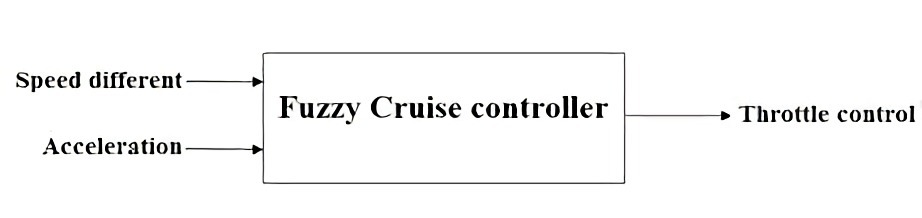
\includegraphics[scale=1.75]{block_diagram}
	\captionof{figure}{Greg Viot's fuzzy cruise controller}
\end{center}

\newpage
\section*{}

\textbf{Theory:} \\

\noindent
G-V controller is used to maintain a vehicle at the desired speed this system consists of two fuzzy inputs namely speed ditference and acceleration and one fuzzy output, namcly throtle control. as shown in \emph{figure 1}.\\

\noindent
Degree of Membership for fuzzy set of input and output is calculated by membership Function given below.

\[
degree\ of\ membership= 
\begin{cases}
0										& \text{if }  delta < 0\ or\ delta \leq 0 \\
min(delta1*slope1,\ delta2*slope 2)	& \text{otherwise}
\end{cases}
\]
\[
where,\ delta1\ =\ x-point1\, delta2\ =point2-x
\]

And, graphically represented as
\begin{center}
	\vspace{0.1cm}
	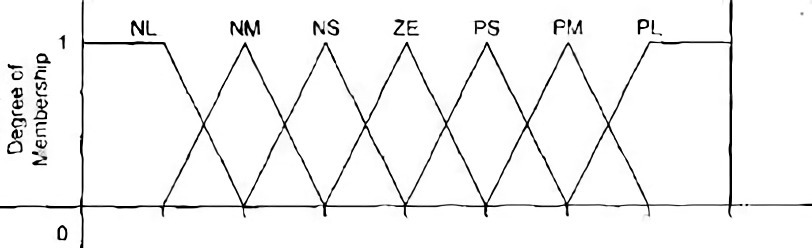
\includegraphics[scale=1.75]{membership_function}
	\captionof{figure}{Memership function}
\end{center}

Here, ZE = Zero, PS, PM, PL are positively small, medium and large respectively also NS, NM and NL
represent negatively small, medium and large respectively. \\

\noindent
Rule base consider in this controller are as follows: \\

\begin{tabular}{| c | c |}
	\hline
	Rule 1  & If (speed difference is NL) and (acceleration is ZE) then (throttle control is PL) \\ 
	\hline
	Rule 2 & If (speed difference is ZE) and (acceleration is NL) then (throttle control is PL) \\ 
	\hline 
	Rule 3 & If (speed difference is NM) and (acceleration is ZE) then (throttle control is PM) \\   
	\hline
	Rule 4 & If (speed difference is NS) and (acceleration is PS) then (throttle control is PS) \\   
	\hline
	Rule 5 & If (speed difference is PS) and (acceleration is NS) then (throttle control is NS) \\   
	\hline
	Rule 6 & If (speed difference is PL) and (acceleration is ZE) then (throttle control is NL) \\   
	\hline
	Rule 7 & If (speed difference is ZE) and (acceleration is NS) then (throttle control is PS) \\   
	\hline
	Rule 8 & If (speed difference is ZE) and (acceleration is NM) then (throttle control is PM) \\   
	\hline
\end{tabular}


\newpage
\section*{}

\textbf{Implementation and Results:} \\

\noindent
1. Input(s):
\begin{itemize}
	\item $speed\ difference \in [-100,\ 100] $
	\item $acceleration \in [-40,\ 40] $
\end{itemize}
2. Output(s):
\begin{itemize}
	\item $throttle \in [-20,\ 20] $
\end{itemize}

\noindent
\linebreak
3. Implementation of speed difference \& acceleration membership functions:
\begin{center}
	\vspace{0.1cm}
	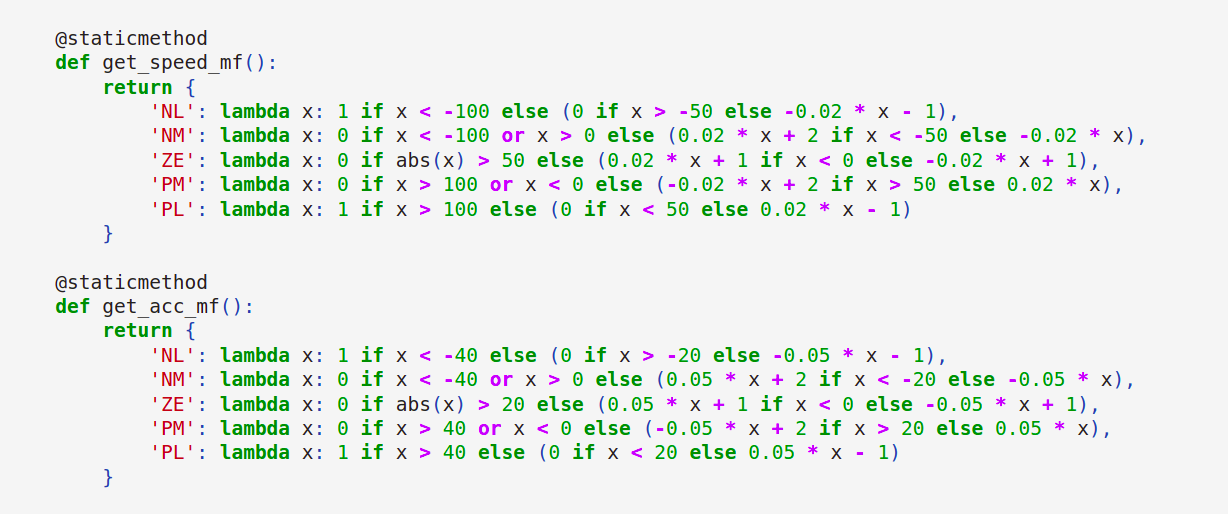
\includegraphics[scale=0.4]{membership_functions}
	\captionof{figure}{Membership function methods}
\end{center}

\noindent
\linebreak
4. Results
\begin{center}
	\vspace{0.1cm}
	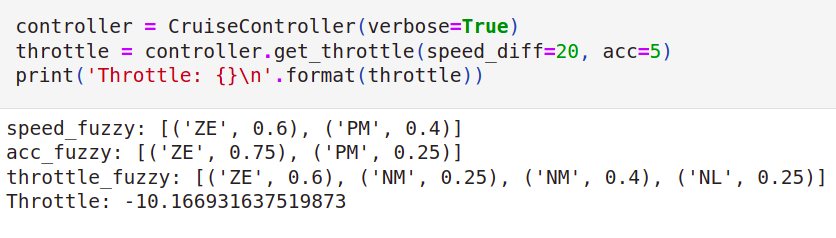
\includegraphics[scale=0.5]{throttle_prediction}
	\captionof{figure}{Throttle position adjustment}
\end{center}

\newpage
\section*{}

\begin{center}
	\vspace{0.1cm}
	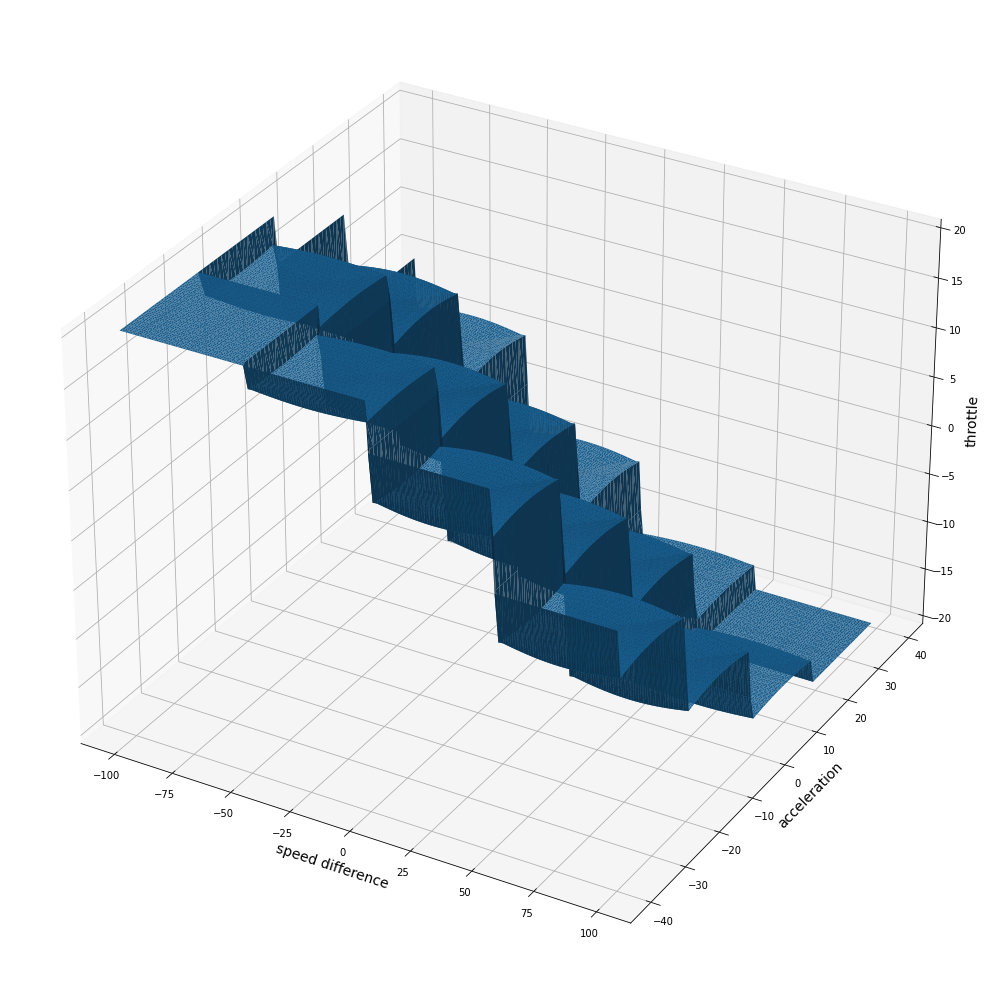
\includegraphics[scale=0.45]{throttle_graph}
	\captionof{figure}{Throttle position based of speed difference, accelration}
\end{center}

\noindent
\\
\textbf{Conclusion:} \\
With this study, we have demonstrated the application of fuzzy logic for designing Greg Viot's fuzzy cruise controller and observed the prediction of throttle adjustment for varying speed difference and instantaneous acceleration. \\


\end{document}

